%%% Results %%%
\chapter{Results} \label{ch:results}
This chapter presents the evaluation criteria for the endorsement model
proposed in chapter ~\ref{ch:method}. Based on which, the overall system design
and functionality will be evaluated and final results will be presented. 

\section{Evaluation Criteria}
Since the purpose of the thesis was only a PoC design, experimental testing on
a real network was not performed. The testing involved a private blockchain
network for the beginning phase and contract deployment was tested on Ethereum
test network, Rinkeby.  To assess the fulfillment of requirements, a
descriptive approach based on the design evaluation method of
\cite{hevner2010design} is used. The system is not only reliant on the smart
contract code and its execution but also on the interaction theory discussed.
For this, the endorsement interaction will be simulated using an interaction
graph simulation tool neo4j. It will follow with the study of graph topology
and relevant subgraphs to study the interactions and base the results on it.
For this interaction, an existing dataset from SNAP\cite{snapnets} is used.
Given the time constraints, no form of structural/unit testing was performed.
However, manual testing was done in parallel with implementation using truffle
and remix ide where necessary. Additionally, front-end for the simple
endorsement interaction was also deployed to test simple function calls and
communicate from the web browser itself. 

\section{Fulfillment of User stories and Requirements}
The method to examine fulfillment of user stories and requirement is influenced
by \cite{Bergquist1107612} that uses Hevner's descriptive design evaluation
approach\cite{hevner2010design}. The table ~\ref{table:fulfillment} presents
the motivation for how the PoC fulfills the functional requirements.\\ 

The fulfillment of non-functional system requirements is discussed below:\\
\textbf{SmartContract Security:} Given the limited timeframe of this project
($\sim{4}$ months), not all security considerations were taken into account. As
part of fail-early principle(footnote), the contracts function code was ordered
as conditions, actions, interactions where relevant. A snippet of a function to
demonstrate this is presented below. 

\begin{lstlisting}[language=Solidity]
	function joinNetwork(string _userName) public{
		//conditions: only allow unregistered participant
		require(!joined[msg.sender]);

		//actions
		joined[msg.sender] = true;
		
        //Interaction
		Participant memory newParticipant = Participant({
				identifier: msg.sender,
				name: _userName
        });
		participants.push(newParticipant);
        LogJoinNetwork(msg.sender, $_$userName);
        numberOfParticipants++;
        participantIndex[msg.sender] = numberOfParticipants-1;
    }
\end{lstlisting}

\begin{center} \label{table:fulfillment} 
	\begin{table}
		\begin{tabular} {| l | l | p{9cm} | }
		\hline
		\textbf{User}  & \textbf{Traceability}   & \textbf{Motivation for fulfillment} \\
		\hline
		\multirow{2}{*}{Endorser} & R1 & Any registered participant can make a
		call to endorse() function to send an endorsement to other registered
		participants on the network.      
		\\\cline{2-3} 
		& R2  & Any registered participant can call removeEndorsement()
		function just by providing the address of the endorsee they wish to
		remove.  \\\cline{2-3}
		& R3 & Each call to endorse() function updates the state variable of
		the current endorser and endorsee, storing and updating the respective
		state variables. i.e., nEG, nER, index. This function call also invokes
		updateEndorsee() function to update the endorsee information
		accordingly.  \\\cline{2-3}
		\hline
		\multirow{2}{*}{Endorsee} & R5.& The storage of personal information
		was not fully implemented by the endorsement PoC, therefore, editing
		personal information is irrelevant. However, change to pseudonym can be
		possible by just making a call to editName() by the participant.
		\\\cline{2-3}
		\hline
		\multirow{2}{*}{other users} & R4.1 & Anyone can make a call to
		computeImpact() function to get the final computed score of a
		participant based on public key hash registered on the endorsement
		network. \\\cline{2-3}
		& R4.2 &  Anyone can make a call to joinNetwork() function and become a
		registered participant of the network immediately.  \\\cline{2-3}
		\hline
	\end{tabular}
	\caption{Fulfillment of User stories and Requirements for Endorsement PoC}
\end{table}
\end{center}

\textbf{Reliability:} The reliability attribute refers to the tamper-proof,
immutable traceability and verifiable nature of data. The blockchain
infrastructure fulfills this requirement. The data in the context of
Endorsement PoC is the endorsement interaction, list of endorsers and endorsees
and the last computed endorsement impact of the respective user, etc. On a PoW
setup, miners, the reliance is on miners to collect and put forward the list of
transactions to the block. As long as a malicious attacker does not own more
than 50\% of the processing power, PoW as a consensus mechanism is considered
safe. The transactions once collected by miners and sent to the blockchain can
be safely assumed to stay there as an immutable set of records. 



\textbf{Trust metrics correctly describe the actual trust of the nodes:} For
this requirement, an interaction graph is simulated, and different scenarios
are modeled that represents different possible behavior in the network.  Refer
to section ~\ref{sec:interaction} for this.



%%%%%%%%%%%%%%%%%%%%%%%%%%%%%%%%%%%%%%%%%%%%%%%%%%%%%%%%%%%%%%%
\section{Interaction graph} \label{sec:interaction}
For the simulation of user interaction in endorsement network and the resulting
impact value, a real-world data set was used. The dataset was extracted from
Bitcoin Alpha trust  \footnote{https://alphabtc.com/blockchain/} weighted
signed network which was mainly a who-trusts-whom network of people that trade
on Bitcoin Alpha platform. Participants on this network rated each other on a
scale of -10 to +10 where negative value represented total distrust whereas
positive value represented total trust. It consists of 3,783 nodes that made
24,186 edges out of which 93\% of the edges were marked as positive
edges\cite{kumar2016edge}.\\
\begin{figure}[h]
	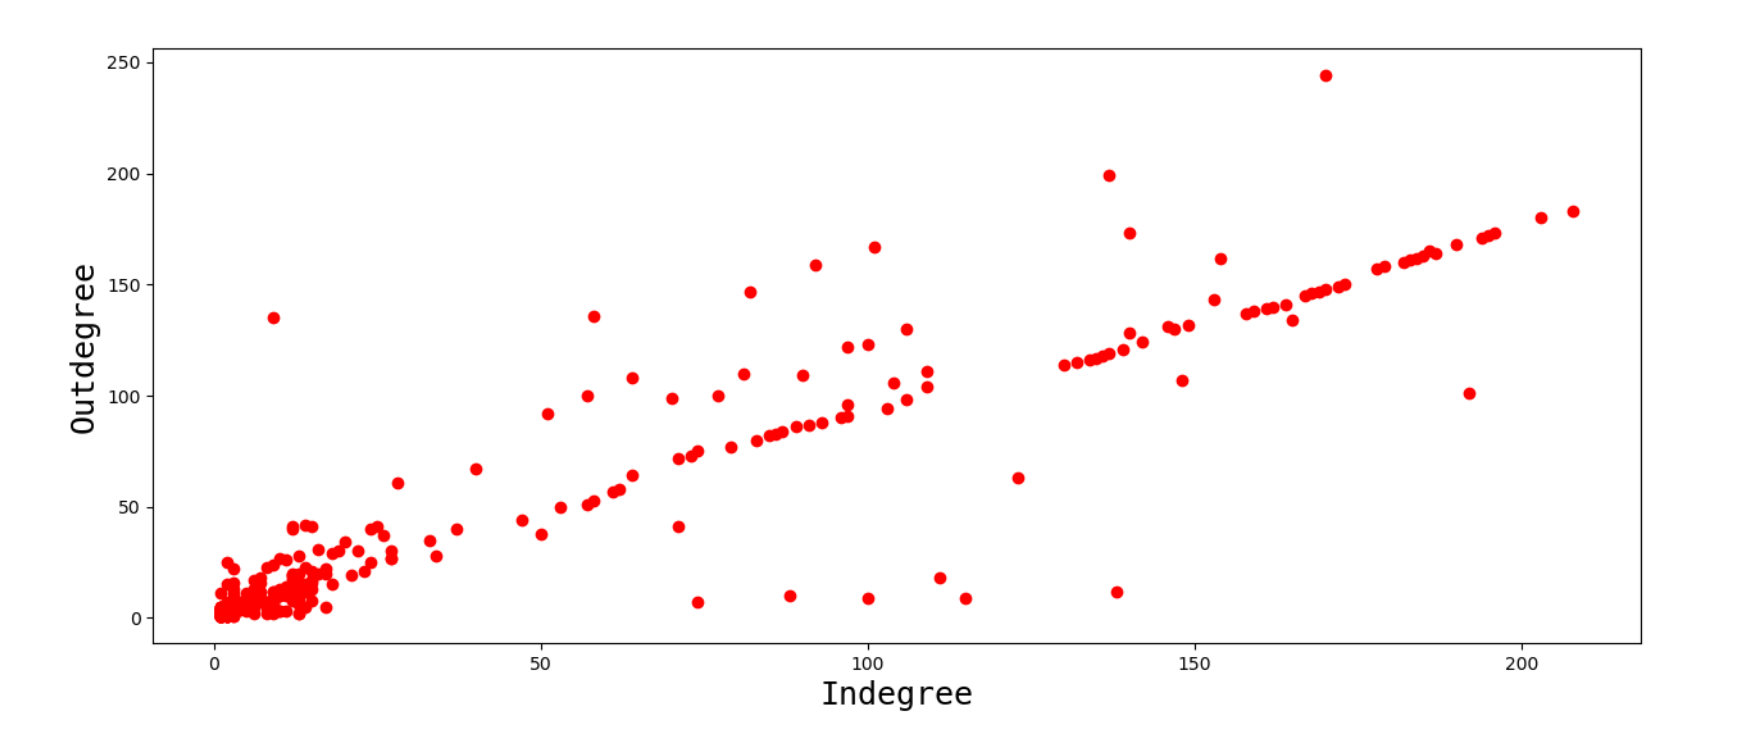
\includegraphics[width=0.95\textwidth]{Images/in_out.eps} 
	\caption{Given Vs. Received} 
	\label{inOut}
\end{figure}

The available information in the dataset for all the nodes was source, target,
rating, and timestamp. All of which is essential information for endorsement
network. The direction of endorsement is based on the source and target
information. The timestamp is also essential information when using a network
anomaly detection algorithm such as net flow rate convergence(cite). The rating
shows the strength or weakness of the relation. 
Unlike the Bitcoin Alpha network that let users rate on a scale of -10 to +10
to demonstrate the strength of their trust towards other users. The endorsement
is more of a boolean decision problem. i.e., A user either endorses a specific
claim made by the entity or doesn't endorse. There is no range of values to
depict the strength or weakness. For the sake of making it a bit more relevant
to endorsement interaction, the existing dataset was filtered only to have
edges with a rating above +2. No negative edges were considered for the
endorsement simulation. As a result, the total number of nodes was reduced to
1677 with 4776 edges. \\
An attempt was made to compute the total endorsement impact of all these nodes
based on their edges relation. The scores along with new findings are presented
below: \\
Total Endorsement Impact: This value is based on the degree of connections and
total received points for each node. Surprisingly, there were 1175 nodes(70\%)
whose final computed score was equivalent to zero. On examining the nodes, it
was found that all of these nodes only had one incoming or outgoing
connections. One requirement that was designed to the endorsement model was
that a node needs to have at least 2 or more connections. The distribution of
indegree and outdegree can be seen in figure ~\ref{inOut}. Having one
connection is only considered a start in the network. The zero, in this case,
is not a representation of a non-trustworthy node, but a starting node.
Therefore, it can be assumed that 70\% of the nodes in the network are new
users. This computation leaves the network with only 502 nodes to account for
having a considerable impact value. 
\begin{tabularx}{\textwidth}{| X | X | X | X | X| X| }
  \hline
   \textbf{Node Label} & \textbf{nEG} & \textbf{nER} & \textbf{ratio} & \textbf{ReceivedPoints} & \textbf{Impact} \\
  \hline 
  430  & 5  & 3  & 0.6 & 0 & 0 \\
  \hline
   761 & 2  & 2  & 1 & 0 & 0 \\
  \hline
  448  & 3  & 3  & 1 & 0 & 0 \\
  \hline
  676  & 2  & 2  & 1 & 0 & 0 \\
  \hline
  936  & 2  & 2  & 1 & 0 & 0 \\
  \hline
  \caption{Nodes with Impact zero because of the receivedpoints}
  \label{table:receivedpoints}
\end{tabularx}

\textbf{Received Points:}
The remaining 502 nodes had connections more than 1. Nevertheless, there were
still few nodes among them with impact value equivalent to zero. This is due to
another factor, received points, that the endorsement impact takes into
account. The relation between Total received points, and total endorsement
impact is shown in figure ~\ref{fig:receivedpointvsimpact}. The received point
is more or less representative of a prestige centrality metrics in a graph
network.  i.e., the node's significance is dependent on the significance of
other nodes it is connected to. However, in case of endorsement network,
Determines the significance of a node based on the significance of other nodes
it is connected to. This factor is more or less similar to the prestige
centrality metrics in a graph network. However, in this case, the significance
is not directly associated with the total endorsement impact of the node it is
connected to. Instead, the depleting consumable point of a giving node
accumulates to the received points to a receiving node. 
The interaction subgraph is shown in figure ~\ref{fig:zeroimpact} for the
discussed nodes behavior. The figure makes it clear that even though the nodes
430, 761, 448, 676, 936 have a degree of connection that is more than 1, their
respective endorsers do not. Table ~\ref{table:receivedpoints} displays the
state and scores of these nodes. 
\begin{figure}[h]
	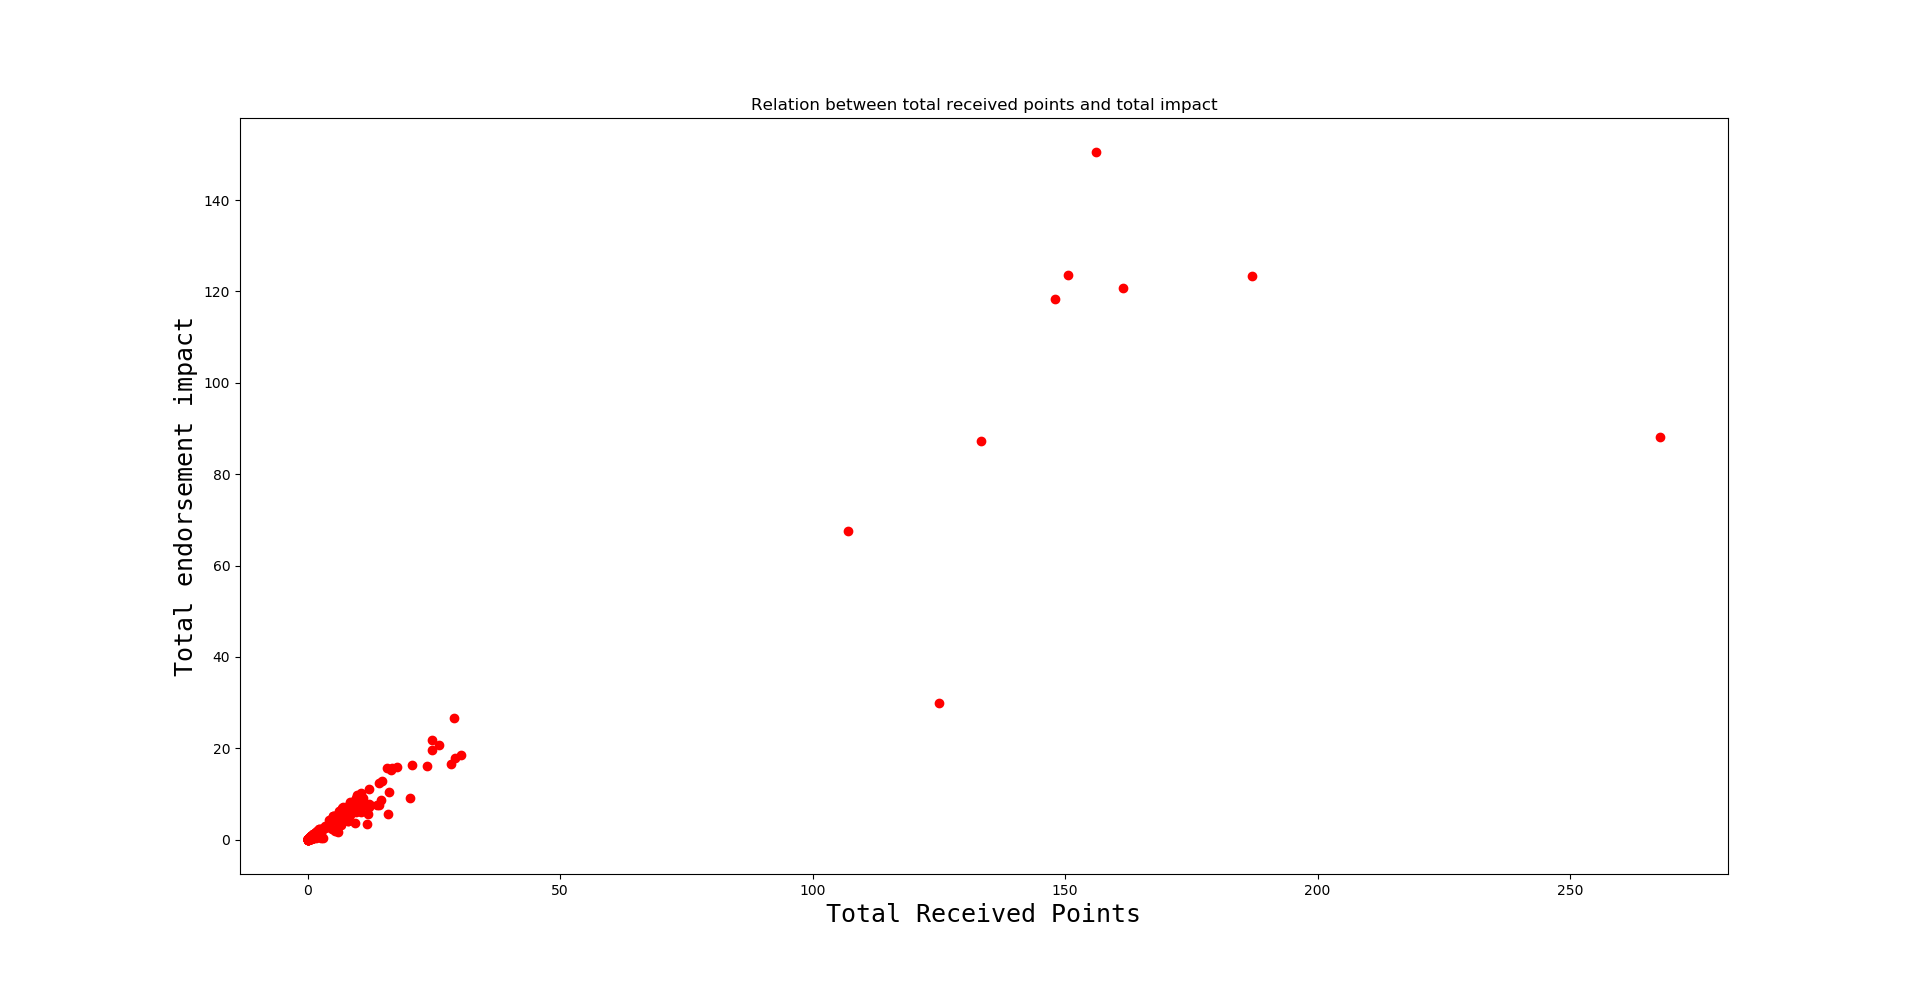
\includegraphics[width=0.95\textwidth]{Images/receivedPoints_impact_impactAboveZero.eps}
	\caption{Received Points Vs. Total Endorsement Impact}
	\label{fig:receivedpointvsimpact}
\end{figure}


\begin{figure}
	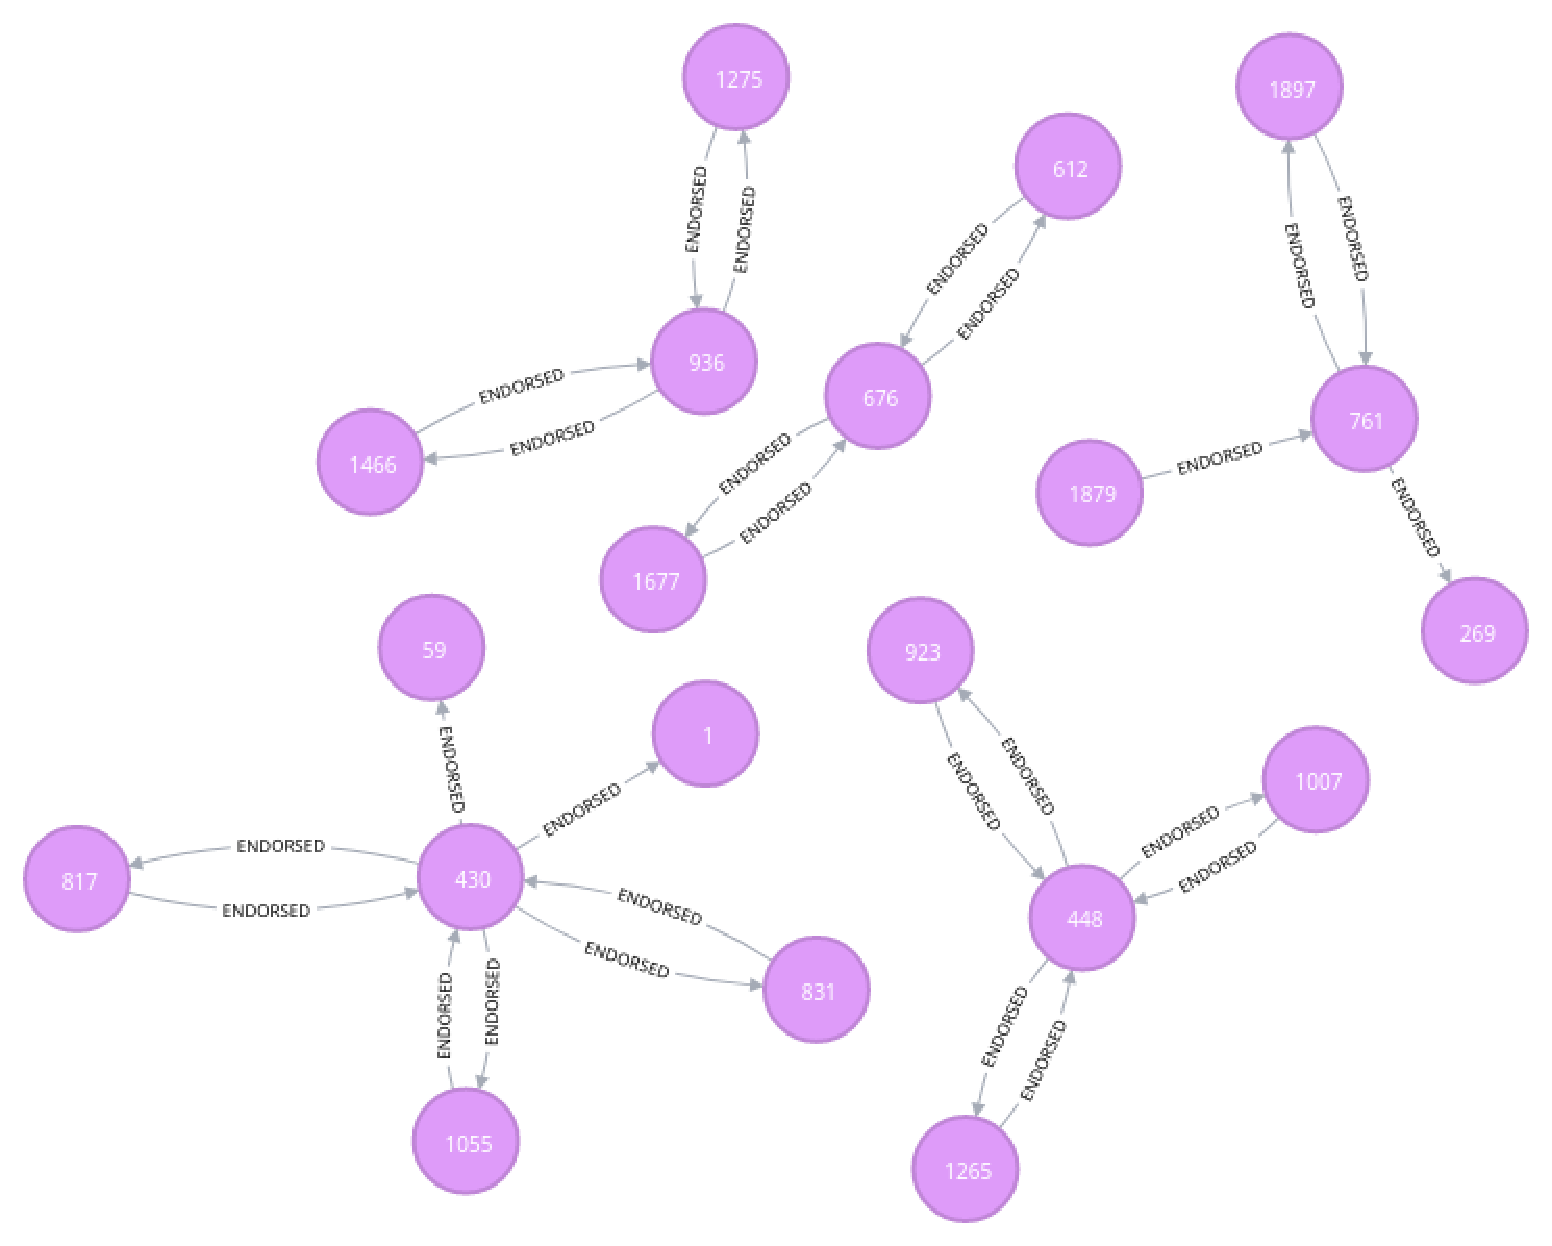
\includegraphics[width=0.95\textwidth]{Images/nodesWithImpactZero.eps}
	\caption{Interaction subgraph of nodes with impact zero}
	\label{fig:zeroimpact}
\end{figure}
\textbf{Ratio:}
Another significant factor that the Impact computation takes into account is
the ratio of indegree and outdegree. The table \ref{table:receivedpoints} makes
it clear that ratio alone is not enough to have a high impact. The figure
~\ref{fig:ratioimpact} shows the relation of ratio and total endorsement impact
over all nodes. One can infer that higher ratio does not imply a higher impact
but a higher impact most probably implies a higher ratio. As such, it is a
contributing factor in the long run. 
\begin{figure}[h]
	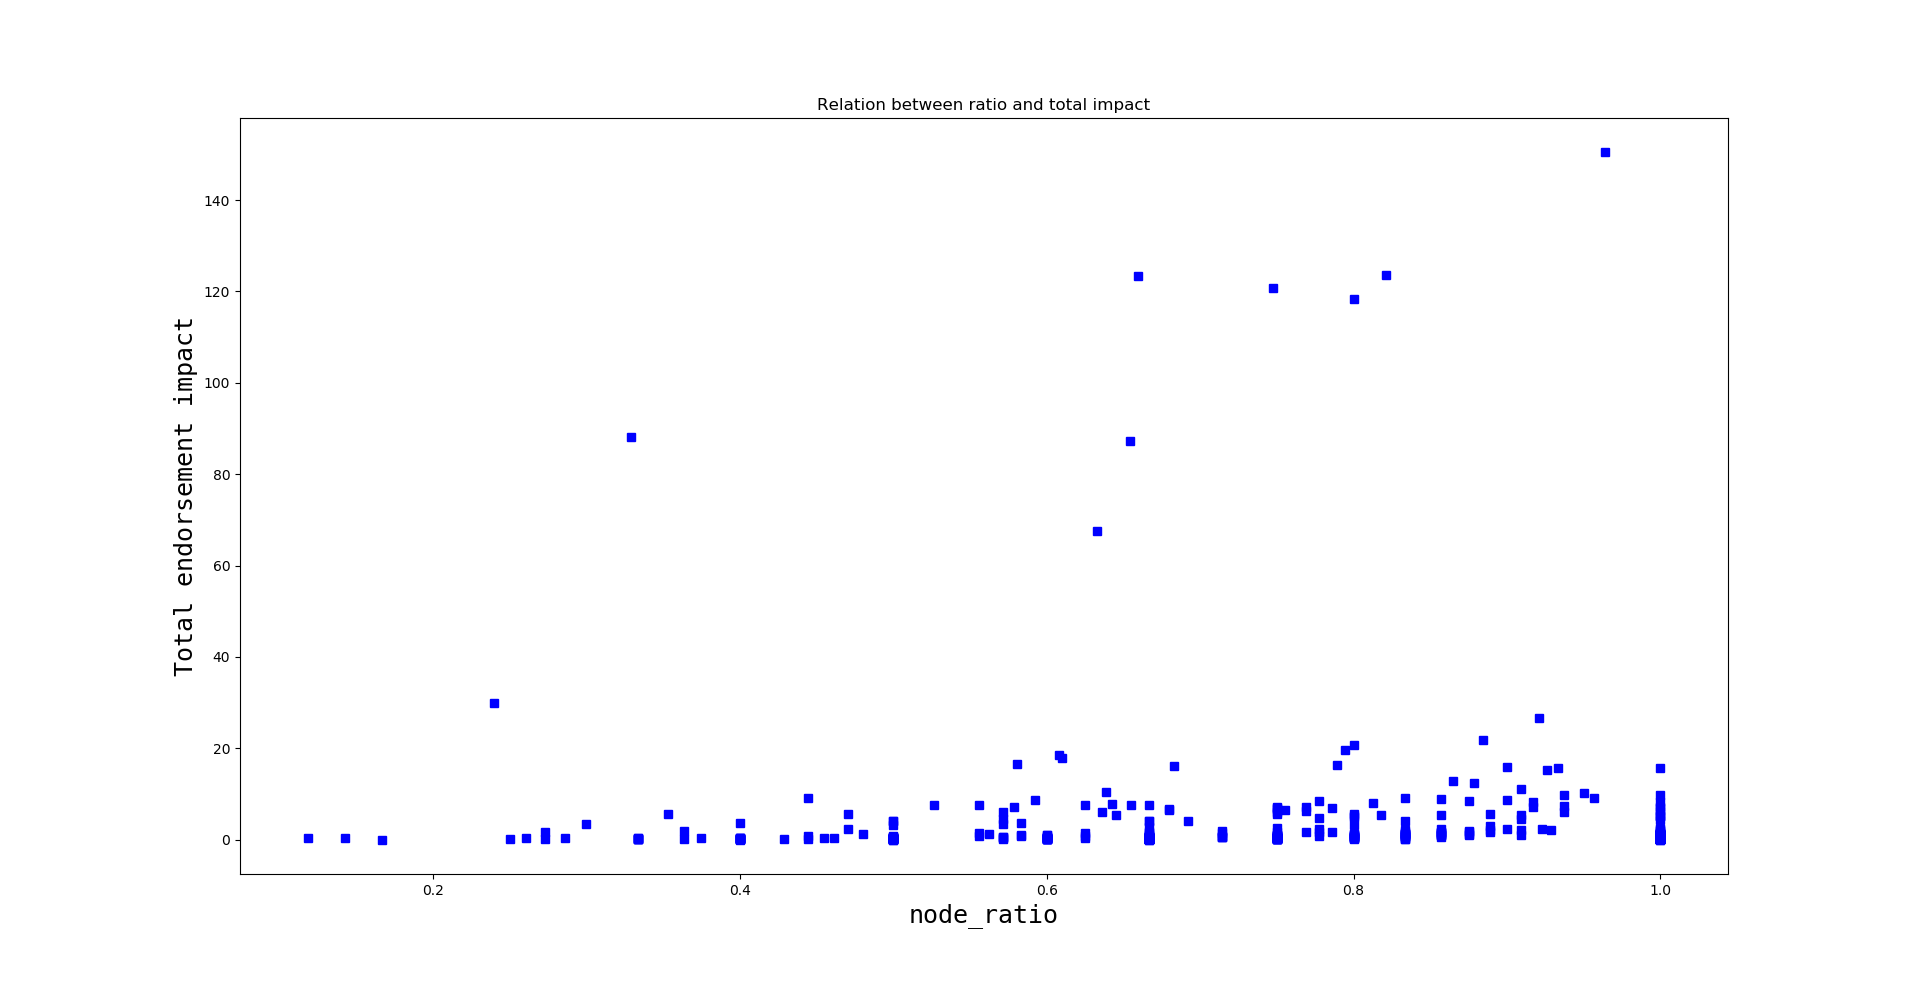
\includegraphics[width=0.95\textwidth]{Images/ratio_impact_impactAboveZero.eps}
	\caption{Relation of Ratio and Total endorsement impact}
	\label{fig:ratioimpact}
\end{figure}
Among the nodes that have maintained an above zero value for total endorsement
impact, the distribution of ranges is shown in table ~\ref{table:totalimpact}.
Majority of nodes have impact value within the range of 0-25. Only a few nodes
have managed to obtain a higher impact value.  For simplicity, one could
classify the impact value ranges as less trustworthy, average trustworthy and
more trustworthy. Based on the distribution table ~\ref{table:totalimpact},
0-55, 55-105 and 105-155 can be used for the mentioned classification. The term
maximum impact henceforth refers to the more trustworthy nodes, average impact
to average trustworthy and minimum impact refers to less trustworthy nodes. 

\begin{tabularx}{\textwidth}{| X | X | }
  \hline
   \textbf{No. of nodes} & \textbf{Impact Range} \\
  \hline 
  419  & 0-5  \\
  \hline
   51 & 5-10 \\
  \hline
  5 & 10-15 \\
  \hline
  10 & 15-20 \\
  \hline
  2 & 20-25 \\
  \hline
  1 & 25-30 \\
  \hline
  1 & 30-35 \\
  \hline
  0 & 35-65 \\
  \hline
  1 & 65-70 \\
  \hline
  0 & 70-85 \\
  \hline
  2 & 85-90 \\
  \hline
  0 & 90-115 \\
  \hline
  1 & 115-120 \\
  \hline
  3 & 120-125 \\
  \hline
  0 & 125-150 \\
  \hline
  1 & 150-155 \\
  \hline
  \caption{No. of nodes and the corresponding impact ranges}
  \label{table:totalimpact}
\end{tabularx}
\section{Total impact across several factors with different scenarios}
Different scenarios are considered to clarify further the relationship between
ratio and total endorsement impact. It seeks to answer the question such as why
a high ratio can both contribute to a high and low total endorsement impact and
vice-versa. Although only these two factors are mainly focused on creating
different cases, the study will show the effect of other factors and their
state as well. 
\subsection{Case1: Maximum Impact, Minimum Ratio}
All the nodes that got maximum impact value when computing the endorsement
impact are considered in this case. Among them, the nodes with the low ratio
are extracted to examine the behavior. As can be seen in figure
~\ref{fig:case1}, the lowest ratio of a maximum impact node is 0.6. This
illustrates the behavior mentioned earlier that a maximum impact node most
certainly has a maintained ratio. 
\begin{figure}
	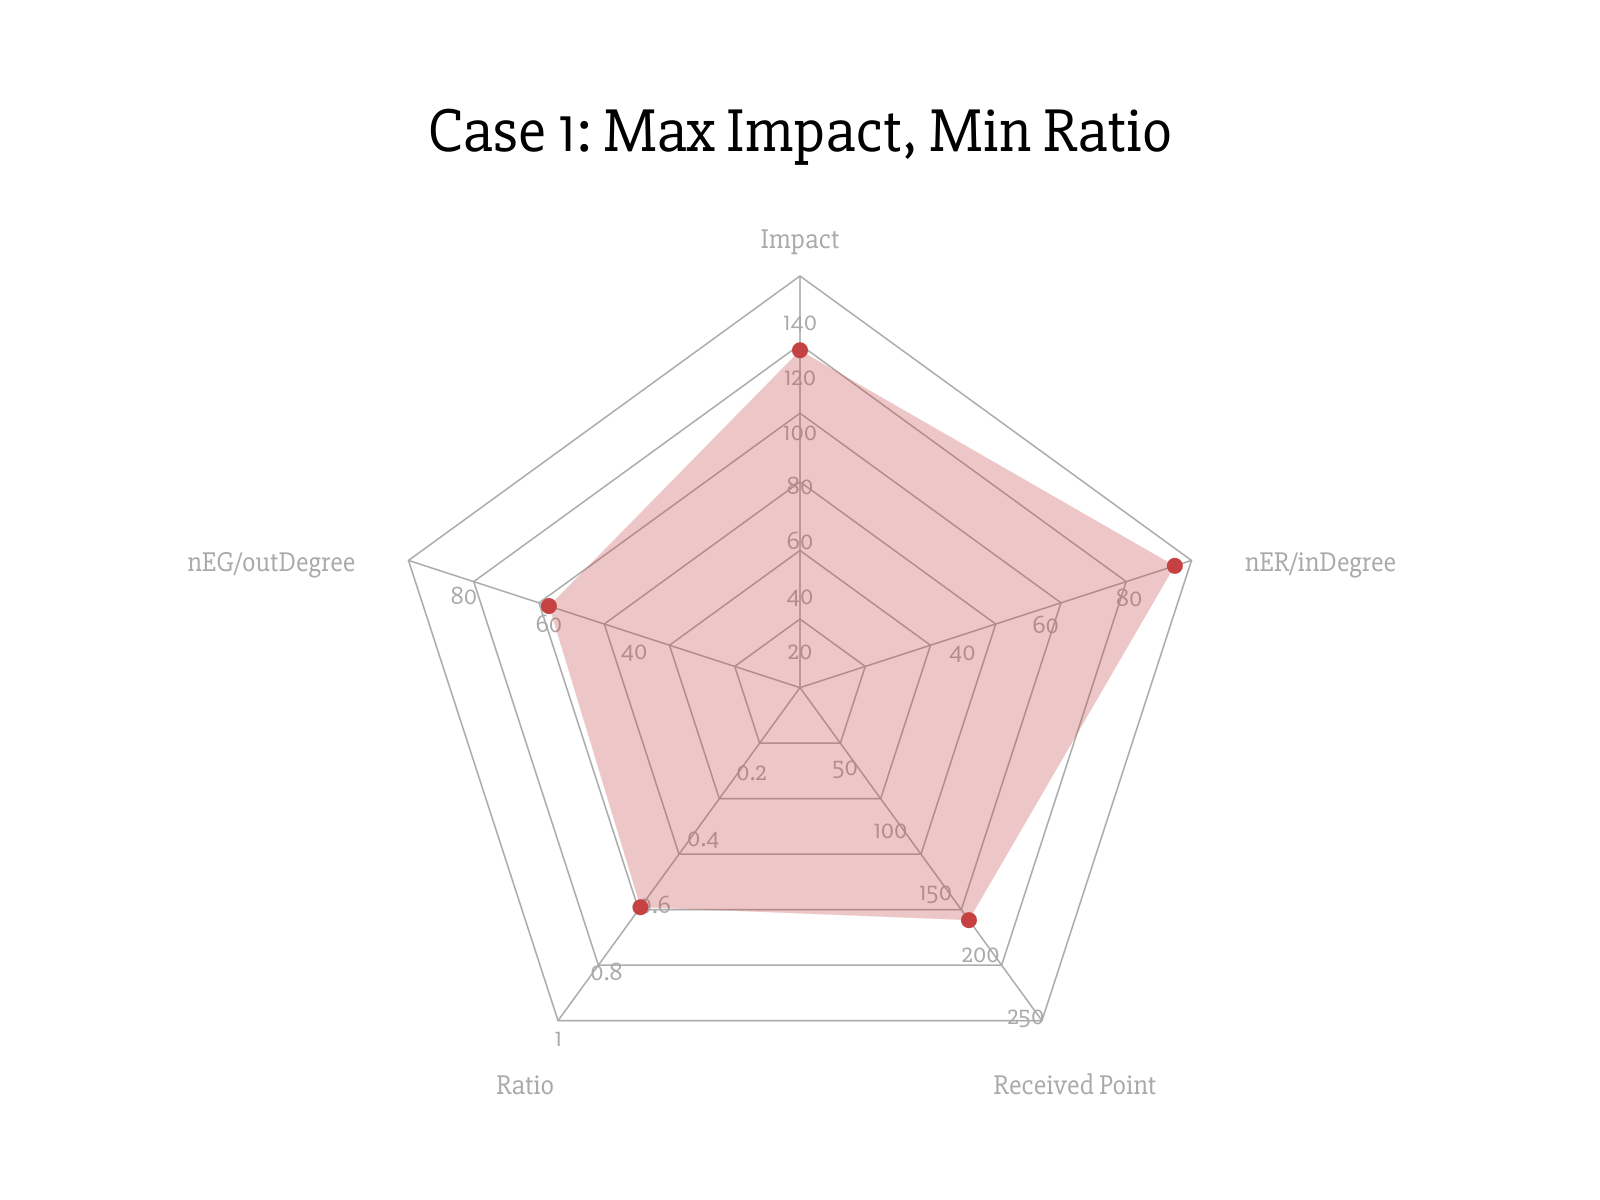
\includegraphics[width=0.95\textwidth]{Images/case-1-max-impact-min-ratio.eps}
	\caption{Case1- Maximum Impact Minimum Ratio}
	\label{fig:case1}
\end{figure}
\subsection{Case2: Maximum Impact, Maximum Ratio}
A maximum ratio of a node with a maximum impact should be the maximum ratio
possible in the network. This behavior is the best case scenario where a node
is actively participating both as an endorser and an endorsee. The data is
taken using the same approach as in case1 for this scenario as well. The
behavior of such a node is depicted in figure ~\ref{ fig:case2}. The value
across all dimension is equally distributed. 
\begin{figure}[h]
	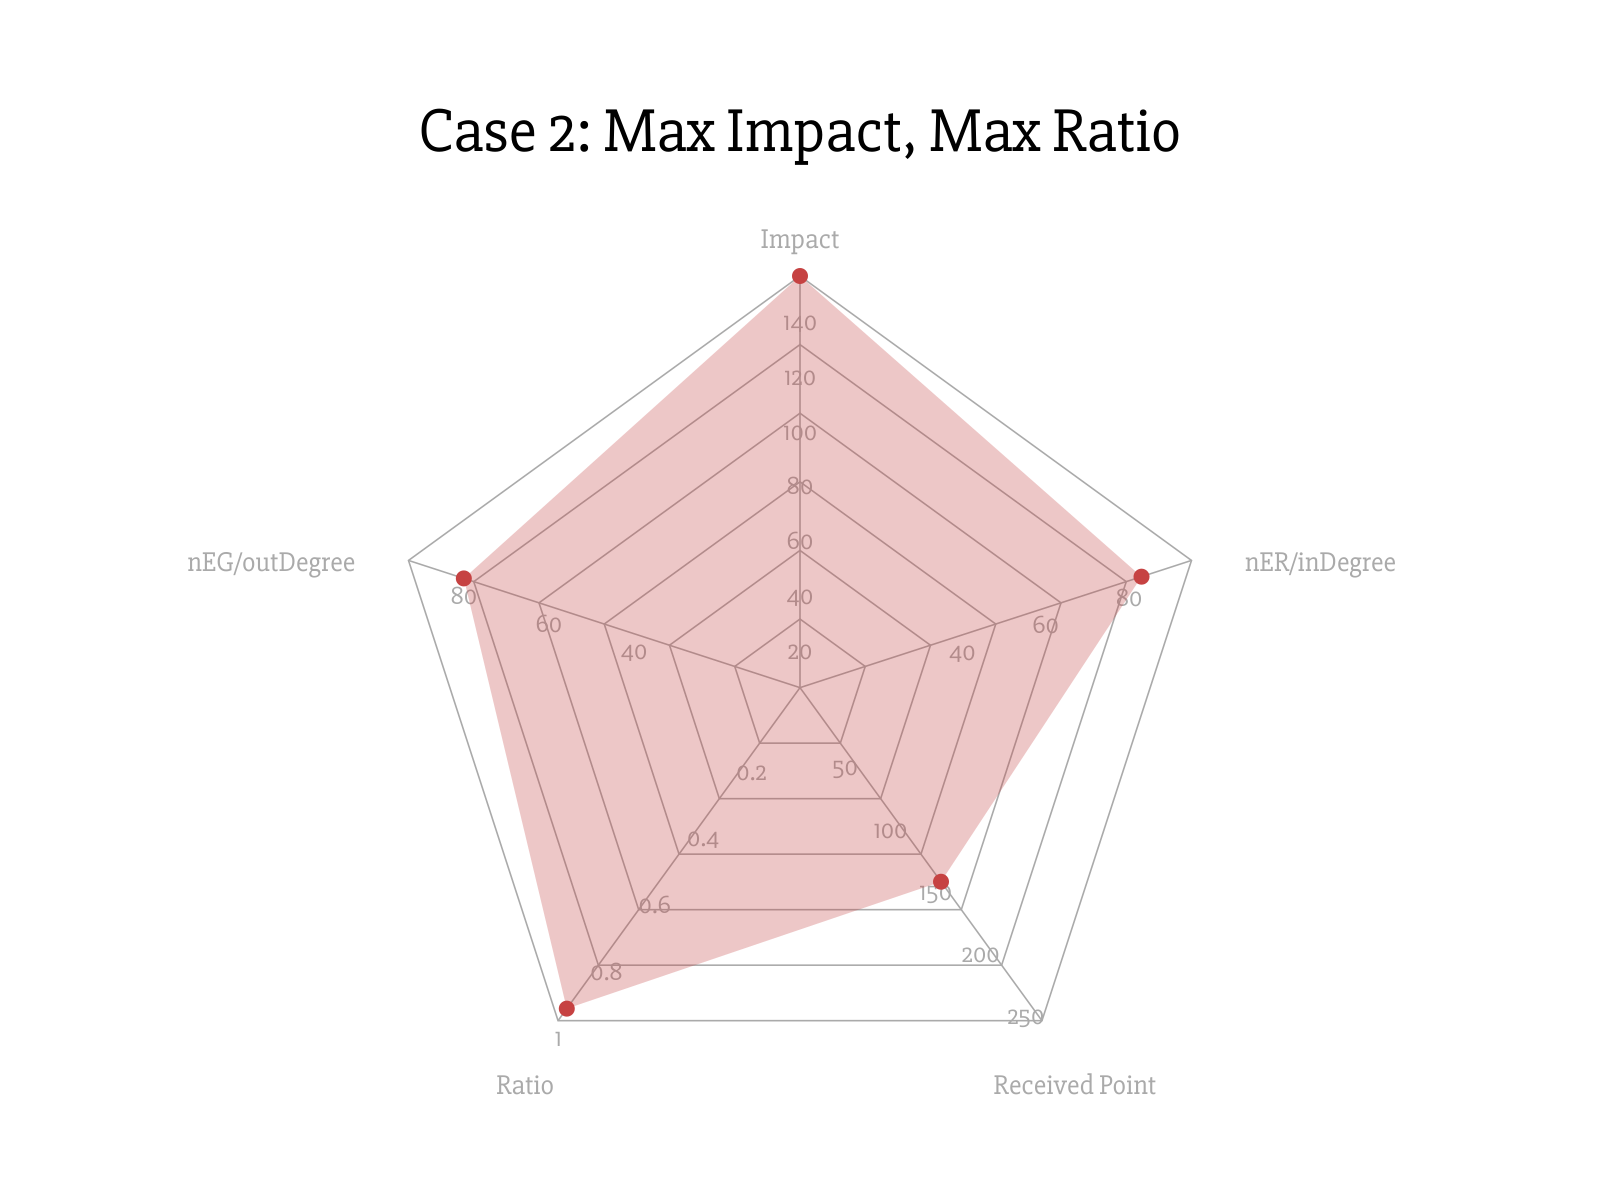
\includegraphics[width=0.95\textwidth]{Images/case-2-max-impact-max-ratio.eps}
	\caption{Case2- Maximum Impact Maximum Ratio}
	\label{fig:case2}
\end{figure}
\subsection{Case3: Minimum Impact, Minimum Ratio}
A minimum impact node is the one that is not an active participator in the
network across all dimension as required. For this category, all the nodes from
minimum impact region were taken. From those nodes, the node with the minimum
impact is taken to show the behaviour as shown in figure ~\ref{fig:case3}. It
can be seen that the node has only actively involved in giving out endorsements
but received relatively low connections. As such, neither the ratio or the
impact is significant for this node. This behavior is typical of an extreme
one-way connection. 
\begin{figure}[h]
	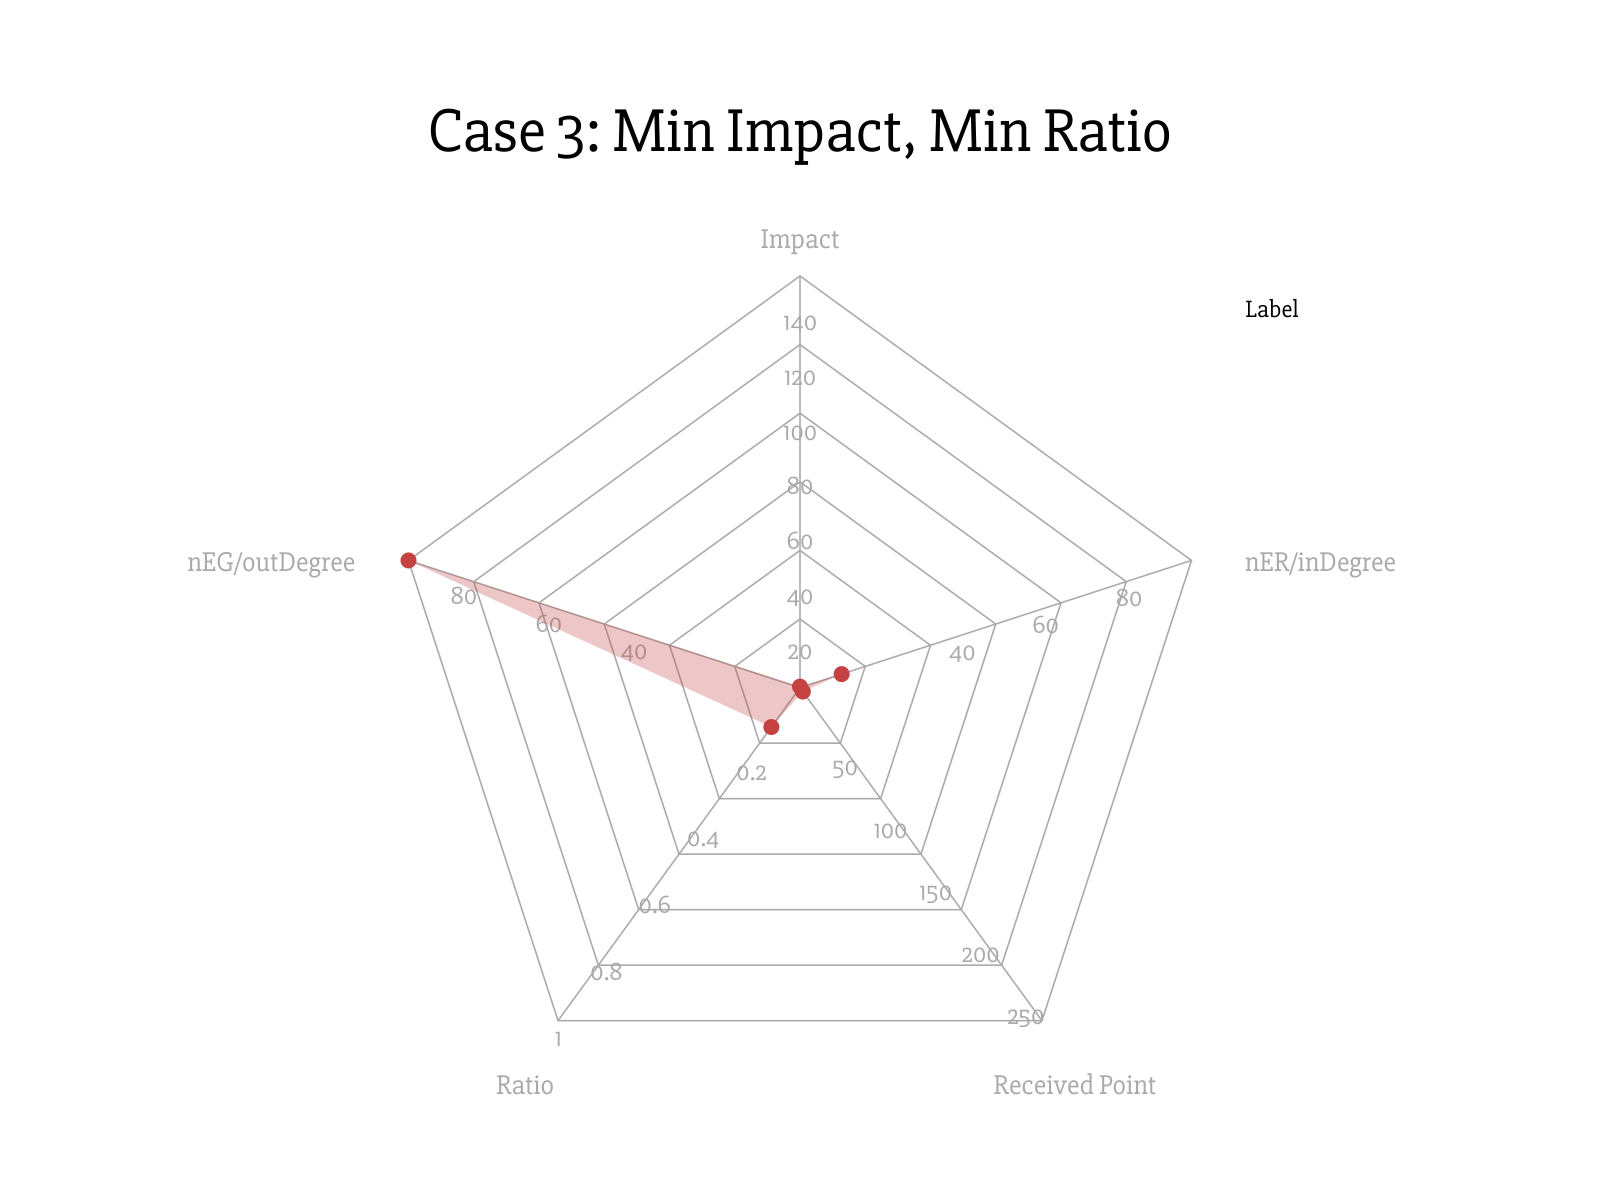
\includegraphics[width=0.95\textwidth]{Images/case-3-min-impact-min-ratio.eps}
	\caption{Case3- Minimum Impact Minimum Ratio}
	\label{fig:case3}
\end{figure}
\subsection{case4: Minimum Impact, Maximum Ratio}
Table ~\ref{table:receivedpoints}  and figure ~\ref{fig:ratioimpact} has
already demonstrated this form of behavior as well. From the minimum impact
nodes, the node with the maximum ratio is taken to simulate an interaction that
looks like figure ~\ref{fig:case4}
\begin{figure}
	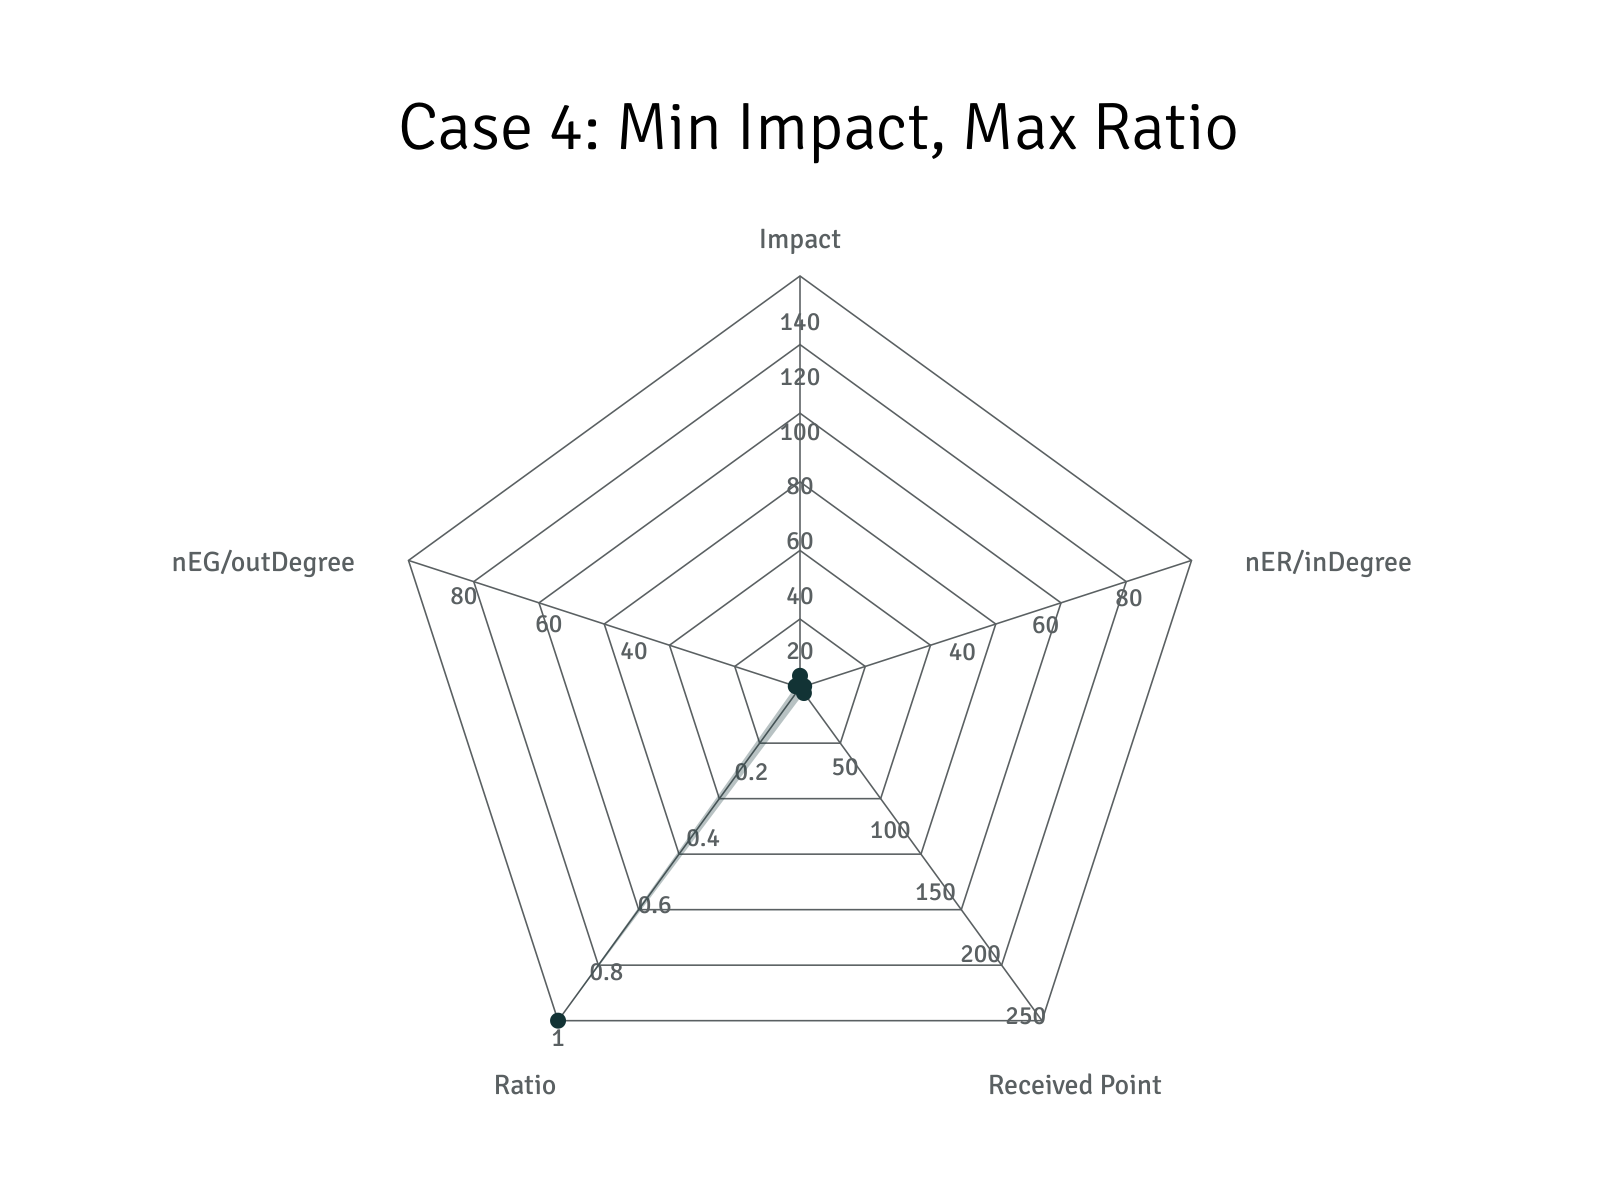
\includegraphics[width=0.95\textwidth]{Images/case-4-min-impact-max-ratio.eps}
	\caption{Case4- Minimum Impact Maximum Ratio}
	\label{fig:case4}
\end{figure}


%\section{Analysis}
%\section{Measurement}
%\section{Comparison}

% Presentation of results and case-study data 
% An application of the methodology is unfolded and results are presented using for example via Charts, Diagrams, Figures and Tables 
% The work is conducted in accordance with the method described earlier. Results are presented in an analytical way.
